\section{Design}
When designing a tool for parsing large input files and applying flexible configuration alternatives,
there are quite a few aspects that needs to be considered. Through this section the design choises
briefly explained in \autoref{subsec:design_choises} will be further explained and more deeply understood.

PET has to be designed for good performance.


\begin{figure}
    \includegraphics[width=0.9\textwidth]{figs/pet-pipeline-gv.pdf}
    \caption{PET-pipeline}
    \label{fig:pipeline}
\end{figure}

put UML-figures here
trådpool
concurency
arbeidsdeling
ringbuffer, statisk vs. ikke statis størrelse



\section{Input}
New hardware architectures are not easily analysed without physical
implementation, but often we are able to simulate its behaviour to acceptable
accuracy, and thus we are able to test different implementations with low cost.
These simulation runs can often be set up to produces trace logs which contains
a user controlled amount of detail. PET can use these trace logs and scan them
for predefined events, each affecting the power consumption of the simulated
hardware. Different simulators have different trace log formats and different
trace abilities. We have chosen gem5 as our target simulator as it is easy to
configure, and trace is well implemented. As mentioned in
\autoref{subsec:design_choises} other options are available, but the support for
easily configurable CPU- and memory system along with the pre-implemented ARM
processors and in-department hands-on experience with this simulator made gem5
the most logical choise.

\subsection{gem5 trace logs}
When run with \texttt{--debug-flags=Bus,Cache,MemoryAccess,Exec} gem5 will output trace files look like
the text displayed in \autoref{lst:trace}.

\begin{lstlisting}[basicstyle=\tiny,caption={gem5 trace log},label={lst:trace},escapeinside={@}{@},float]
@\label{line:physmem}@3021: system.physmem: Write of size 8 on address 0x82fe0 data 0xe1a0f00eee1d0f70
@\label{line:icache}@3021: system.cpu.icache: access for ReadReq address 9c0 size 64
@\label{line:cachemiss}@3021: system.cpu.icache: ReadReq (ifetch) 9c0 miss-
...
@\label{line:cacheupdate}@3432: system.cpu.dcache: Block addr 81f0 moving from state 0 to state:7 valid: 1
3432: system.cpu.dcache: Leaving recvTimingResp with ReadResp for address 81f00
3432: system.tol2bus.respLayer1: The bus is now busy from tick 234320 to 236376
@\label{line:memread}@1642: system.cpu T0 : 0x89d4.0 : ldr   r1, [sp] #4     : MemRead :  D=0x00000000
@\label{line:intalu}@1642: system.cpu T0 : 0x89d4.1 : addi_uop   sp, sp, #4 : IntAlu :  D=0x00000000b
1701: system.cpu T0 : 0x89d8   : mov   r2, sp          : IntAlu :  D=0x00000000b
1701: system.cpu T0 : 0x89dc.0 : str   r2, [sp, #-4]!  : MemWrite :  D=0x0000000
1760: system.cpu T0 : 0x89dc.1 : subi_uop   sp, sp, #4 : IntAlu :  D=0x00000000b
1760: system.cpu T0 : 0x89e0.0 : str   r0, [sp, #-4]!  : MemWrite :  D=0x0000000
4000: system.membus: recvTimingResp: src system.membus.master[0] ReadResp 0x1640
4000: system.l2: Handling response to ReadResp for address 1640
4000: system.l2: Block for addr 1640 being updated in Cache
\end{lstlisting}

Each line in \autoref{lst:trace} represents an event that happens in the
simulated hardware.  \autoref{line:physmem} tells that a write access to
physical memory has happened. \autoref{line:icache} is the event of instruction
cache access, while \autoref{line:cachemiss} shows that this request failed.
During this simulation, there is also events like \autoref{line:cacheupdate}
which represents that the data cache updates some content. The discrete
instructions running through the CPU is also logged, eg. \autoref{line:memread}
shows a load-instruction and \autoref{line:intalu} shows an
addition-instruction.

As discrete events are picked out from the trace logs, PET accumulates power
consumption in equally sized timeslots, called buckets. Each bucket has a
parameter controlled size in terms of simulator ticks. Often it is more
practical to specify the number of buckets in the output rather then specifying
the number of simulator ticks in each bucket. Because of this, PET is able to
estimate the bucket size by peeking at the tick at the last line of the trace
file. It has been shown that the trace file is not nessesary in tick order,
but it will commonly be at approximatly the last tick at the last line. The
bucket size estimation algorithm is shown in \autoref{alg:bucket_size}.

\begin{algorithm}
    \caption{Bucket Size Detection Algorithm}
    \label{alg:bucket_size}
    \begin{algorithmic}
        \Function{numTicks}{$traceFile$}

        \State $eofPos \gets \Call{getSize}{traceFile}$
        \State $\Call{seek}{traceFile, eofPos - 3}$
        \State
        \State $char \gets \Call{getChar}{traceFile}$
        \While{$char \ne newline$}
            \State $\Call{seek}{traceFile, -1}$
        \EndWhile
        \State $line \gets \Call{getLine}{traceFile}$
        \State $simulatorEvent \gets \Call{parseLine}{line}$
        \State \Return $\Call{getTick}{simulatorEvent}$
        \EndFunction
    \end{algorithmic}
    \begin{lstlisting}[language=Python]
function numTicks( traceFile ):
    # Find file size
    eof_pos = traceFile.getSize()

    # Seek almost to end, avoid last newline
    traceFile.seek( eof_pos - 3 )

    # Trace from back of file to second last newline
    while not traceFile.currentChar is '\n':
        traceFile.seek_backwards

    # File stream position is now at beginning of last line
    # Parse this line
    simulatorEvent = parseLine( traceFile.getLine() )

    # Return the tick of the retreived event
    return simulatorEvent.getTick()
    \end{lstlisting}
\end{algorithm}

\autoref{lst:trace} also shows that the events in the trace log is not nessesary in their
correct order, thus PET has to be able to add power consumption to the entire timeline at all
time. This means that we are unable to produce continous output, but have to store the
results in memory and dump them when the entire input is parsed.


\subsection{PET weight files}
Equally important as finding the correct events is assigning each event the
correct amount of power consumption. As each event will count differently
depending on the architecture, PET will read a weight file along with the gem5
trace log. A sample weight file is listed out in \autoref{lst:weights_example}.
As the timeslots are specified in simulator ticks instead of CPU cycles,
the values have been chosen to match a 2GHz processor, which then means
one CPU cycle pr. 500 simulator ticks using standard gem5 simulation granularity.
If you are applying this method to a processor with a different clock speed than
2GHz, be aware that the numbers has to be scaled propotionally. This is not the
case for the static power drain, as it is simply added to each timeslot, and is
not scaled in accordence with bucket size.

\lstinputlisting[caption={Weight file example},label={lst:weights_example},float,language=Python]{../pet/weights.conf}

The weights displayed in \autoref{lst:weights_example} are assigned and
accumulated each time PET discovers a recognisable event in the log file. A
simplified version of this algorithm can be found in
\autoref{alg:power_accum_algo}

\begin{algorithm}
\caption{Power Accumulation Algorithm}
\label{alg:power_accum_algo}
\begin{lstlisting}[language=Python]
# map of accumulated power for each time step
map<time,power> output

# input is all trace log lines, elements in weight file and
# the determined bucket size (number of simulator ticks in
# each bucket)

function assignWeights( traceLogLines, weightMap, bucketSize )
    # run through each line
    for each line in traceLogLines:
        # extract event parameters from line
        simulatorEvent = praseLine( line )

        # get the assigned weight from weight file
        eventWeight = weightMap[simulatorEvent.getEventType()]

        # add this weight to the output map
        output[simulatorEvent.getTick()/bucketSize] += eventWeight
    return output
\end{lstlisting}
\end{algorithm}
%weightfiles
%

\section{Output}
Depending on application, different output formats might come in handy. PET
supports printing plain time power dump, a somewhat more readable table to
plain, table and a gnuplot figure with time as X-axis and power drain on the
Y-axis. The output format is understood as timeslots in which the architecture
has a certain current drain, which should be multiplied with applied voltage to
get numbers on consumed energy, heat generation and so on. The numbers are
scaled as milliamperes, which of cource is equal to milliwatt if voltage is
$1V$.

Example of the \texttt{plain} output format can be seen in
\autoref{lst:pet_output_plain}. The left column is the bucket number, while the
right column is instant current draw from the modelled architecture.

\begin{lstlisting}[label={lst:pet_output_plain},caption={PET Plain Output}]
0 120
1 113
2 150
3 123
4 133
5 117
\end{lstlisting}

When reading the output directly from console, a more descriptive output format
is the \texttt{table} format. An example using this option is rendered in
\autoref{lst:pet_output_table}.

\begin{lstlisting}[label={lst:pet_output_table},caption={PET Table Output}]
/-------------------------\
|   Bucket   |   Energy   |
|-------------------------|
|          0 | 120.000000 |
|          1 | 113.000000 |
|          2 | 150.000000 |
|          3 | 123.000000 |
|          4 | 133.000000 |
|          5 | 117.000000 |
\-------------------------/
\end{lstlisting}

Visualization is often a good thing when inspecting old or trying to understand new
problems. As it is hard to get a good overview from huge text log files, PET provides
an optionally annotated graphical output. In effect, it is formatting temporary output
files and calling GNUPlot do do the hard work.

\begin{figure}
    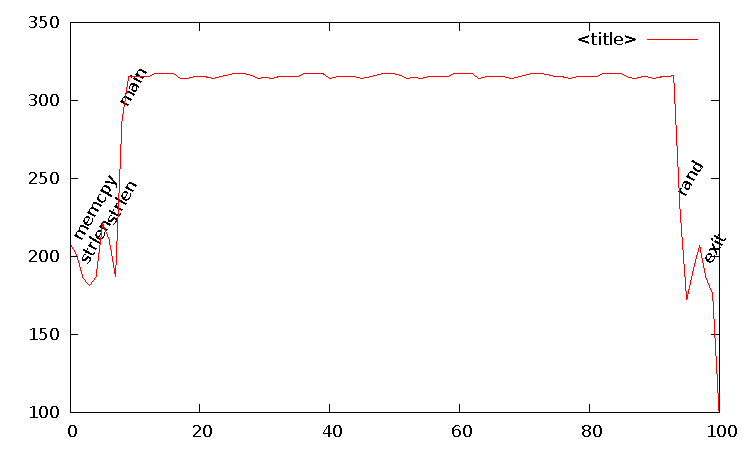
\includegraphics[width=0.9\textwidth]{figs/annot.pdf}
    \caption{PET Annotated Graphical Output}
    \label{fig:annot}
\end{figure}

